%===============================================================================
\section{Planning}
\label{section:planning}

The projects plan in the temporal domain is presented in this section.

%===============================================================================
\subsection{Milestone plan}

See Fig.\:\ref{fig:MileStone} for the milestone plan.

\begin{figure}
    \centering
    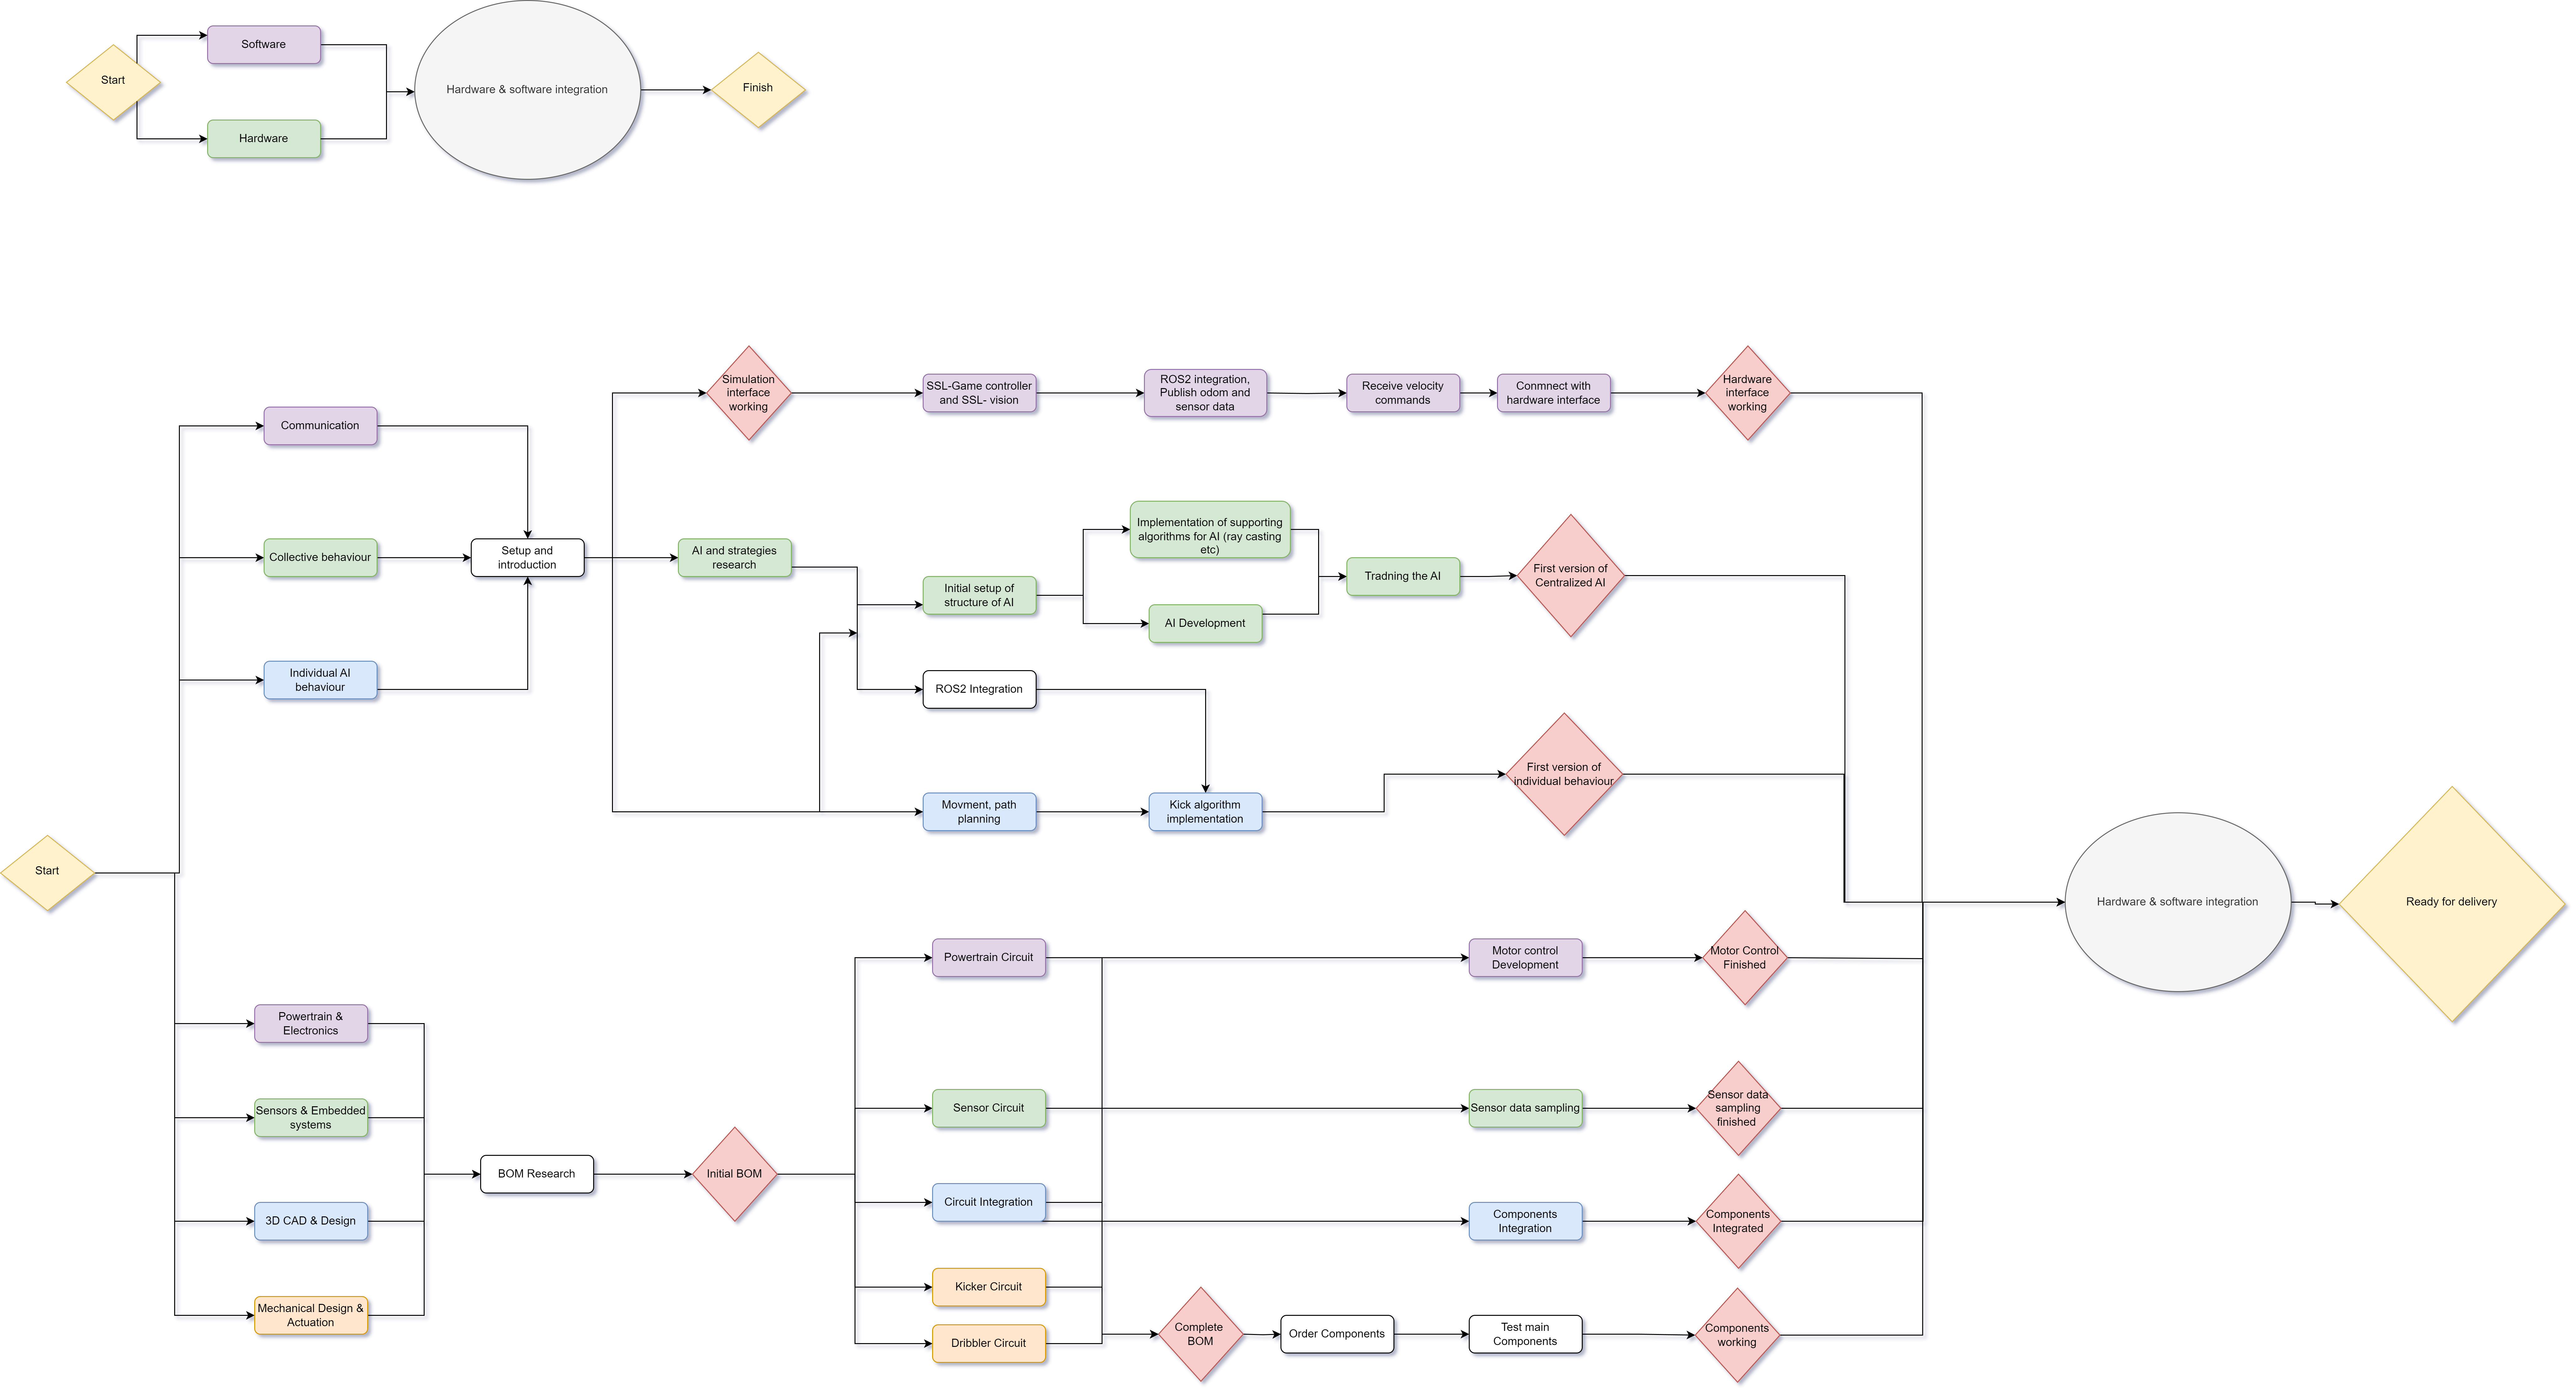
\includegraphics[width=\linewidth]{images/MileStone_for_PRO1.png}
    \caption{The milestone plan for the project.}
    \label{fig:MileStone} 
\end{figure}

%-------------------------------------------------------------------------------

%\helper{Stakeholders may want an overarching flow chart or table of the project’s most important milestones as a indicator if the project is falling behind.}

%===============================================================================
\subsection{Work breakdown structure}

The \ac{wbs} can be seen in Fig.\:\ref{fig:wbs}.

%-------------------------------------------------------------------------------

\begin{comment}
The Work Breakdown Structure (WBS) is a fundamental tool in project management, establishing a systematic and structured approach to break down the intricate project into manageable components. This detailed, hierarchical decomposition of the project's scope presents a visual or textual representation that facilitates an understanding of the project's structure, workflow, and tasks necessary for successful project completion. A key note is that the WBS should only include items related to the project and not the project course, this excludes items such as course assignments as they are not a part of the project, only the course.

If you need an anecdote, picture this: "You are a consultant assigned to help clients develop a Work Breakdown Structure (WBS) for their project. This WBS will outline the project's components, giving a clear roadmap of what is to come. You also have internal tasks like time reports, presentations, and assignments for your consulting firm. However, it is important to remember that these internal duties belong outside the client's WBS. They are part of your job, not the client's project. By keeping the WBS client-specific, you maintain clarity and ensure an effective project management strategy."

The WBS dissects the project into multiple layers for ease of management, separating the work into components, work packages, deliverables, and tasks.

\begin{itemize}
\item \textbf{Components} represent the broad sections or stages of the project.
\item \textbf{Work Packages} are subsets of these components, which can be further broken down into specific deliverables.
\item \textbf{Deliverables} are tangible or intangible goods or services produced in the project. They can be handed over physically or digitally to another person or team, forming the backbone of each work package and contributing substantially to the overall project's progression.
\item \textbf{Tasks} represent the smallest work units necessary to complete each deliverable, providing clear action items for project participants.
\end{itemize}

By enabling systematic project planning, effective resource allocation, and reliable progress tracking, the WBS becomes an invaluable aid in navigating the complexity of projects and driving them towards successful outcomes.

A small text-based example, recommend visual based, of applying a WBS for a mobile autonomous robot development project is illustrated below, and only one component is added to keep it short for the example. This example should provide a more tangible understanding of the WBS and its purpose.

\begin{table}[H]
    \centering
    \begin{tabular}{|l|l|l|}
    \hline
    \textbf{\textbf{ID}} & \textbf{Type} & \textbf{Activity}                                          \\ \hline
    1                    & Root          & Mobile Autonomous Robot Development                        \\ \hline
    1.1                  & Component     & Navigation and Path Planning                               \\ \hline
    1.1.1                & Work Package  & Sensor Integration                                         \\ \hline
    1.1.1.1              & Deliverable   & Sensor Selection Report                                    \\ \hline
    1.1.1.1.1            & Task          & Research Suitable Sensors (LiDAR, RADAR, Ultrasonic, etc.) \\ \hline
    1.1.1.1.2            & Task          & Prepare Sensor Selection Report                            \\ \hline
    1.1.1.2              & Deliverable   & Sensor Installation Manual                                 \\ \hline
    1.1.1.2.1            & Task          & Install Sensors on Robot Chassis                           \\ \hline
    1.1.1.2.2            & Task          & Prepare Sensor Installation Manual                         \\ \hline
    1.1.1.3              & Deliverable   & Sensor Data Fusion                                         \\ \hline
    1.1.1.3.1            & Task          & Develop Sensor Data Fusion Algorithm                       \\ \hline
    1.1.1.3.2            & Task          & Implement and Test Sensor Data Fusion Algorithm            \\ \hline
    1.1.2                & Work Package  & Path Planning                                              \\ \hline
    1.1.2.1              & Deliverable   & Path Planning                                              \\ \hline
    1.1.2.1.1            & Task          & Research Suitable Path Planning Algorithms                 \\ \hline
    1.1.2.1.2            & Task          & Implement Selected Path Planning Algorithm                 \\ \hline
    1.1.2.2              & Deliverable   & Path Planning Testing Report                               \\ \hline
    1.1.2.2.1            & Task          & Test Path Planning Algorithm in Simulated Environment      \\ \hline
    1.1.2.2.2            & Task          & Prepare Path Planning Testing Report                       \\ \hline
    \end{tabular}%
\end{table}
\end{comment}

%===============================================================================
\subsection{Schedule}

The project schedule can be seen in Fig.\:\ref{fig:project_schedule}, with software schedule in Fig.\:\ref{fig:software_schedule} and hardware schedule in Fig.\:\ref{fig:hardware_schedule}.

\begin{figure}
    \centering
    \begin{subfigure}[b]{0.55\textwidth}
       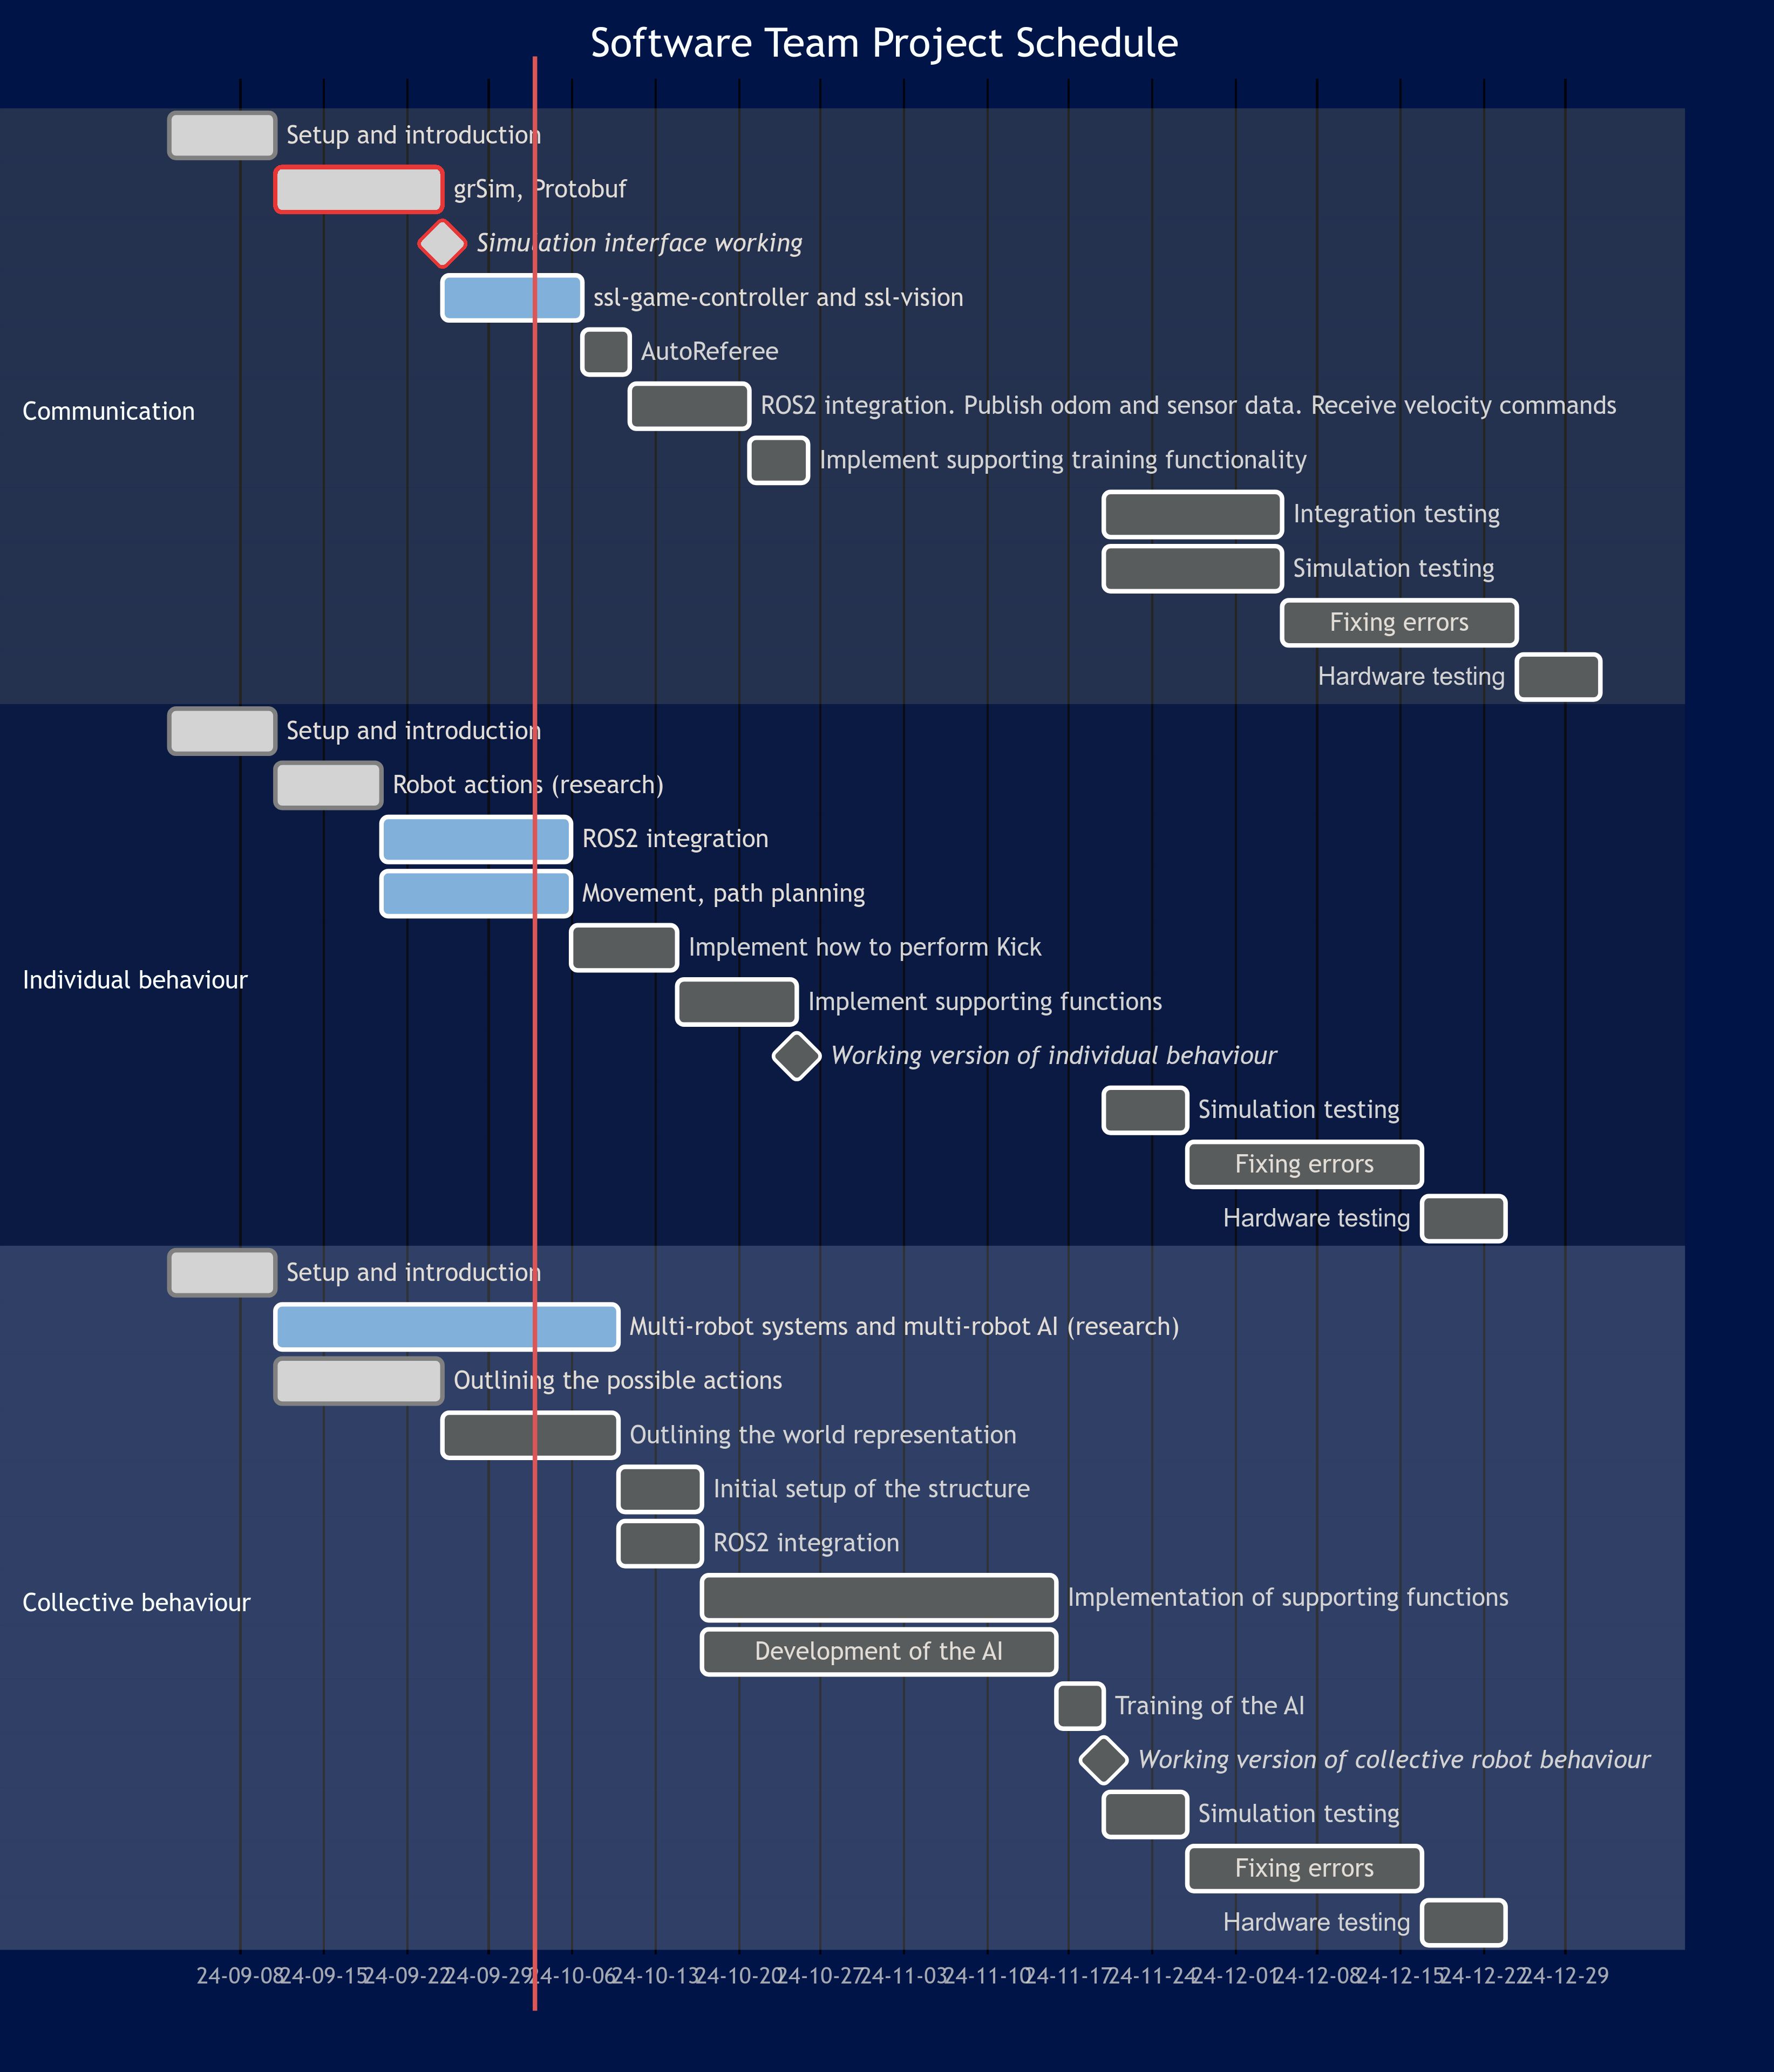
\includegraphics[width=0.95\linewidth]{images/DVA490_software_team_project_schedule.png}
       \caption{Software team schedule.}
       \label{fig:software_schedule} 
    \end{subfigure}
    \hfill
    \begin{subfigure}[b]{0.55\textwidth}
       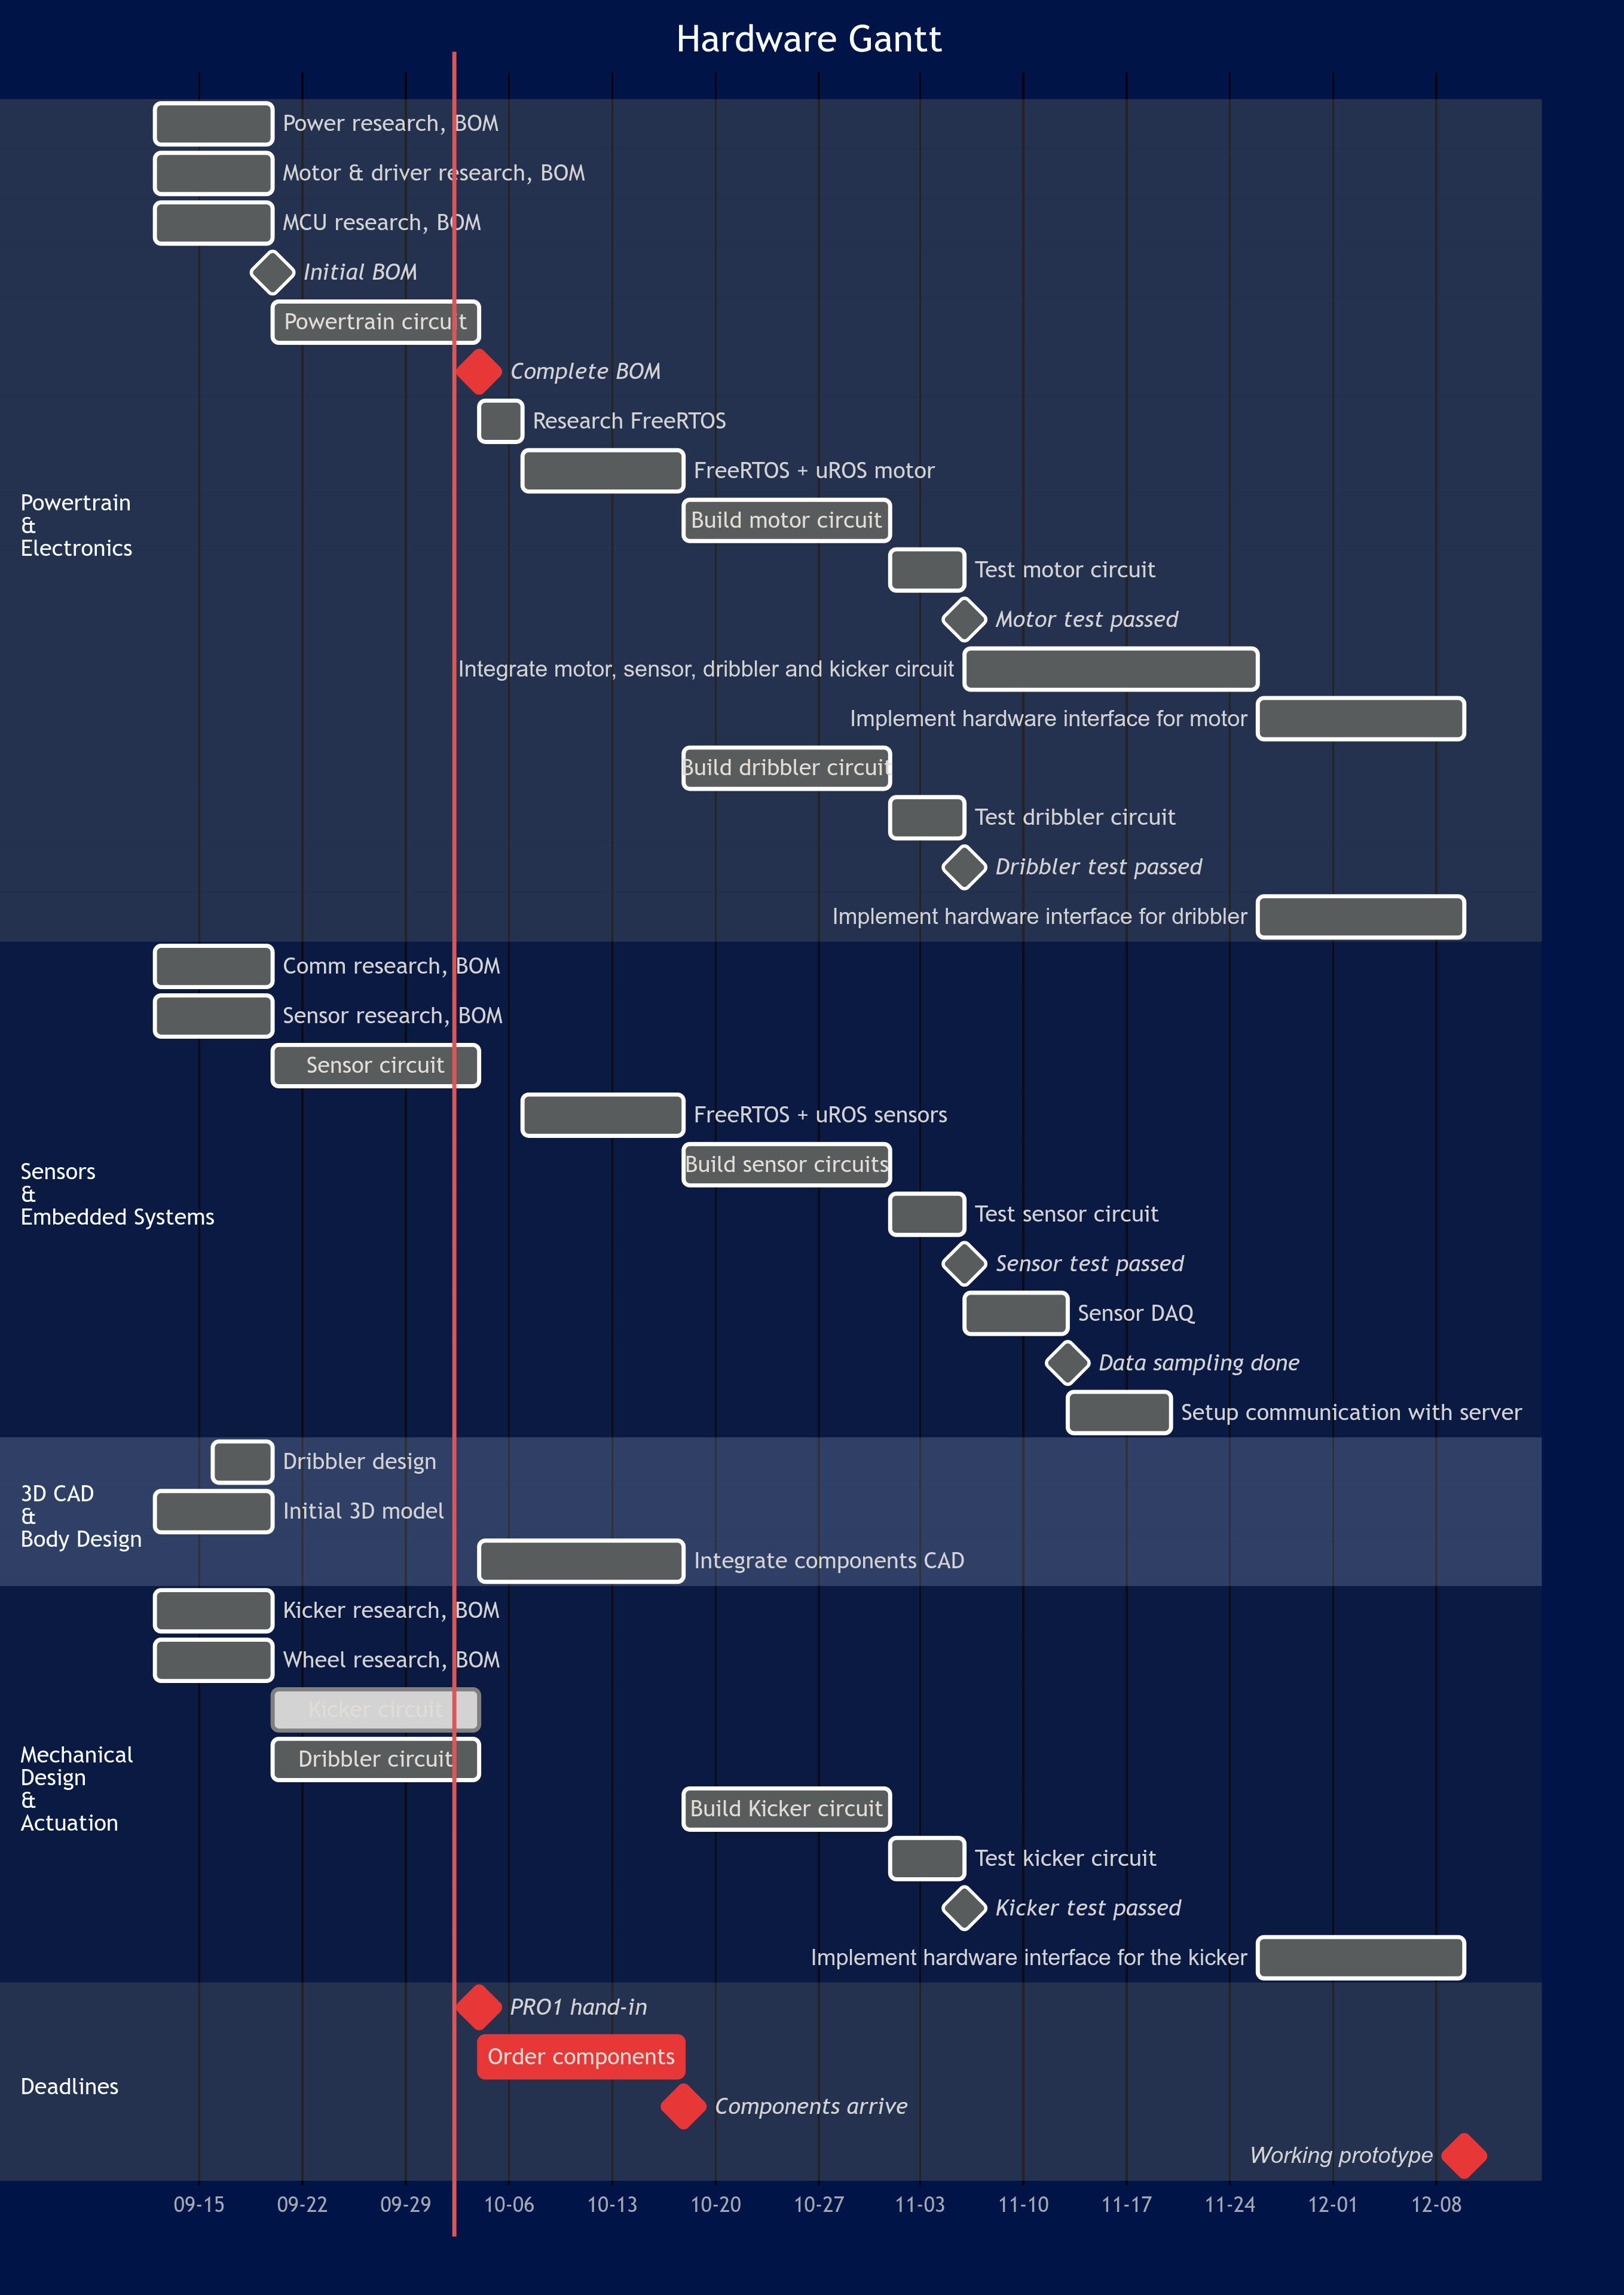
\includegraphics[width=0.95\linewidth]{images/DVA490_hardware_team_project_schedule.png}
       \caption{Hardware team schedule.}
       \label{fig:hardware_schedule}
    \end{subfigure}
    \caption{The project schedule.}
    \label{fig:project_schedule}
\end{figure}

%-------------------------------------------------------------------------------

%\helper{Activity plan with a time axis where duration and connection between activities and milestones are shown.}

%===============================================================================